% Manual template (AAT2), see docs/HowToDoc.md
% Build (in docs/manual):  pdflatex ManualDrumFeatureDemonstrator.tex   (twice, for the references)
% The PDF is copied into the release zips by the GitHub workflow.
\documentclass[12pt]{article}
\usepackage[utf8]{inputenc}
\usepackage[T1]{fontenc}
\usepackage[top=2cm, bottom=2cm, left=2cm, right=2cm]{geometry}
\usepackage{graphicx}
\usepackage{xcolor}
\usepackage{hyperref}
\hypersetup{colorlinks=true, linkcolor=red, urlcolor=red, pdftitle={DrumFeatureDemonstrator Documentation}}

% ---- change these ------------------------------------------------------------
\newcommand{\pluginversion}{0.15.0}   % the version in CMakeLists.txt
\newcommand{\pluginauthor}{Joerg Bitzer}
\newcommand{\sourceurl}{https://github.com/JoergBitzer/DrumFeatureDemonstrator}
% -------------------------------------------------------------------------------

\title{DrumFeatureDemonstrator Documentation}
\author{License: CC-BY 4.0}
\date{\today, for DrumFeatureDemonstrator \pluginversion}

\begin{document}
\maketitle

\section{Introduction}
DrumFeatureDemonstrator is a one-sample drum player with a step grid (1/16 notes, 8 to 32 steps). You load one
sample (a drum hit, a cymbal, a reversed cymbal), choose the steps on which it is played, and change pitch,
direction, loudness, pan and the number of repeats (ratchets) per step. There are four patterns that can be played one after the other,
tools to copy, shift and clear a pattern, and a library of typical patterns. The sample is also played from MIDI notes.

The new thing is \textbf{play to end}. The plug-in knows exactly how long the sample sounds at the chosen
pitch. A step in the mode \emph{reverse + play to end} is therefore started early, so that the sample
\emph{ends exactly at the end of that step}. Put it on the last step before a beat, and a reversed
cymbal leads into the next beat without any manual nudging, at any pitch and any tempo. The plug-in
reads the beat position from the DAW, so it always stays in sync.

\section{Installation}
The downloaded file is a zip file. It contains the plug-in (.vst3; on macOS also the AU,
.component), the Standalone application, a ReadMeFirst.txt, the licence files and this manual.
Copy the plug-in to the right place and let your DAW rescan its plug-ins.

\begin{verbatim}
Windows (VST3):  C:\Program Files\Common Files\VST3
Mac (VST3):      /Users/yourUSERNAME/Library/Audio/Plug-Ins/VST3
Mac (AU):        /Users/yourUSERNAME/Library/Audio/Plug-Ins/Components
Linux (VST3):    /home/yourUSERNAME/.vst3
\end{verbatim}

The macOS version is not signed with an Apple Developer ID. If macOS reports that the plug-in
is damaged or cannot be opened, remove the quarantine flag in the Terminal, e.g.
\texttt{xattr -cr \textasciitilde/Library/Audio/Plug-Ins/VST3/DrumFeatureDemonstrator.vst3}.

\subsection{Presets and settings}
The presets (plain XML files) and the settings file (\texttt{user.settings}: day/night theme)
are stored in this folder -- delete it to remove DrumFeatureDemonstrator completely:
\begin{verbatim}
Windows: C:\Users\yourUSERNAME\AppData\Roaming\Jade_Hochschule\DrumFeatureDemonstrator
Mac:     /Users/yourUSERNAME/Library/Audio/Presets/Jade_Hochschule/DrumFeatureDemonstrator
Linux:   /home/yourUSERNAME/.config/Jade_Hochschule/DrumFeatureDemonstrator
\end{verbatim}

\section{How to use}
\begin{center}
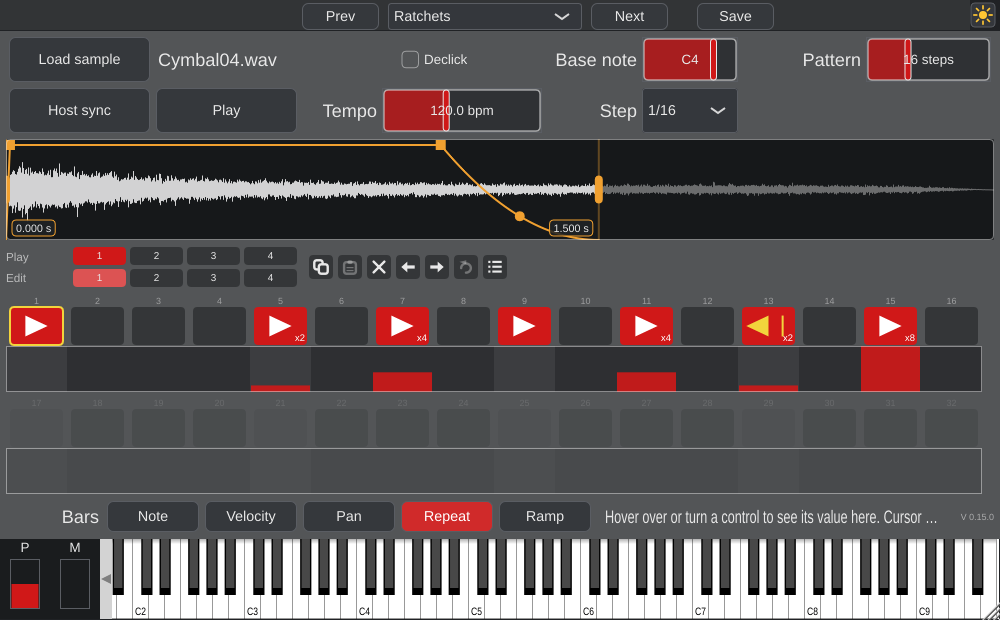
\includegraphics[width=\textwidth]{images/GUI.png}
\end{center}
\begin{enumerate}
    \item \textbf{Load sample}: choose a sample file (wav, aiff, flac, ogg), or drop a file onto the
    waveform. A copy is kept in the folder \texttt{Samples} next to the presets; the sample is stored with
    your DAW project and referred to by its name in a preset.
    \item \textbf{Waveform}: the orange line is the envelope of the played part. Drag the \textbf{start line} and the \textbf{end line}
    (grab the knob in the middle or any point of the lower part of the display) to set start and end; their times in seconds are shown
    next to them. Drag the small squares at the \textbf{top} sideways for the \textbf{fade-in} and \textbf{fade-out time}: the gain rises from 0 to 1
    after the start line and falls to 0 before the end line (the line is slanted accordingly). Both fades together cannot be longer than the played part.
    The small \textbf{circle in the middle of each fade line} bends the fade curve: drag it down for an exponential curve (slow start), up for an
    anti-exponential one (fast start); the straight line in between is linear (a double-click on the circle makes the fade linear again). A small label shows the value while you point at it.
    The plug-in version is shown very small in the bottom right corner.
    With \textbf{Declick} switched on, the start and end line snap to a zero crossing of the sample (no click at the edge).
    \item \textbf{Base note}: the MIDI note at which the sample sits in the scale, i.e. plays at its original speed (C4 = MIDI note 60; range C1 to C5). Changing it transposes all steps and the keyboard.
    MIDI notes (also the keyboard at the bottom) play the sample with the pitch relative to the base note and with velocity.
    \item \textbf{Pattern}: length of the patterns in steps (8 to 32, the same for all four patterns). Steps beyond the length are dimmed.
    \item \textbf{Host sync}: on = the plug-in follows tempo and position of the DAW (it plays while the DAW plays);
    off = internal beat with its own tempo and the \textbf{Play/Pause} button (or the \textbf{space key}).
    \item \textbf{Patterns}: there are four patterns. The upper row of small buttons (\textbf{Play}) switches each pattern on or off for
    playback; the patterns that are on are played one after the other from 1 to 4 (with 1 and 3 on: 1, 3, 1, 3, \dots; the pattern length is
    the same for all). The lower row (\textbf{Edit}) selects the pattern that the step grid shows and edits: it is lit in a brighter red, and a
    \textbf{yellow frame} marks the pattern that plays right now.
    \item \textbf{Steps}: every step has \textbf{one button with four states}. Each click goes one state further: off $\rightarrow$ forward $\rightarrow$
    reverse $\rightarrow$ reverse + play to end $\rightarrow$ off (the symbol shows the state). Below the buttons are the \textbf{bars}: one vertical bar per step,
    side by side. The buttons at the bottom choose what the bars show (the \emph{page}): the \textbf{note} (a MIDI note, shown as e.g. C4; the sample sounds at its
    original pitch when the note equals the base note), the \textbf{velocity} (MIDI velocity 1 to 127) the \textbf{pan} (left -- centre -- right), the \textbf{repeat} (1 to 8 hits within the step, a ratchet; the step button then shows $\times n$) or the
    \textbf{ramp} (how the repeats are spaced: in the middle evenly, above it the hits speed up, below it they slow down; it has an effect with a repeat above 1).
    With reverse + play to end, every repeat ends at the end of its part of the step.
    \textbf{Draw on the bars with the mouse}: press, and drag from left to right (or in any direction): every bar the mouse passes takes the height of the mouse, so a
    line sets all the values at once. A double-click puts a bar back to its default. The yellow frame in the grid shows the step that is playing
    (if the playing pattern is the one shown).
    \item \textbf{Pattern tools} (small buttons right of the pattern buttons, drawn as icons): \textbf{copy} the edited pattern and \textbf{paste} it into the edited
    pattern (also into another one), \textbf{clear} it, \textbf{shift} it one step to the left or right (inside the pattern length; steps that leave come back on the other side),
    \textbf{undo} the last paste, clear, shift or library action, and the \textbf{pattern library}: a menu with typical patterns in the categories BD, SD, HH, Perc and
    Chromatic (the chromatic ones use note offsets from C4). A library pattern replaces the edited pattern; the pattern length and the note value are not changed.
    \item \textbf{Step}: the \textbf{note value} that one step represents, from 1/1 to 1/64, each normal, dotted ($\times 1.5$) or as a triplet ($\times 2/3$). The default is 1/16.
    A pattern of 16 steps of 1/16 is one bar of 4/4; with 12 steps of 1/8 triplets it is one bar of triplets. Play to end ends at the end of the step, whatever its length.
    \item \textbf{Info line} (below the steps): shows the value of the control under the mouse and of the control you change,
    e.g. ``Pattern 1, step 5 note: E4 (MIDI note 64)'' -- there is no room for an edit field per bar.
    \item \textbf{Preset handler} and \textbf{day/night}: as usual; Save turns red when you change a control.
    Presets contain all four patterns, which of them play, the region, the fades and the name of the sample. Factory presets keep the sample you have loaded.
\end{enumerate}

\subsection{Selecting a step and entering notes}
While the transport stands (the DAW is stopped, or the internal beat is paused) the \emph{selected step} is framed in yellow; while
the plug-in plays, the frame follows the playing step. Click into a step (or use the cursor keys: left/right $\pm$1 step,
up/down $\pm$16 steps, Home/End first/last step) to select it. A \textbf{MIDI note} (from the keyboard at the bottom of the window,
or from your MIDI keyboard) sets the \textbf{note and the velocity} of the selected step and switches the step on; the sample
is also heard. The selection does not move by itself; use the cursor keys to go to the next step.

\subsection{Play to end: what to know}
\begin{itemize}
    \item The sound ends at the \emph{end of the step} on which the mode is set. To lead into beat 1, set it on step 16 of a pattern of 16 steps -- with several patterns on, the next beat 1 is the start of the next pattern of the chain (the sound then starts in the time of the pattern before).
    \item If the start time has already passed (the transport starts or jumps into the run-up), the sound is
    \emph{not} played and a notice appears.
    \item Play to end is only possible if the sample (at its pitch) is not longer than the pattern (the number of steps times the length of a step). Otherwise the mode button
    is outlined in red and a notice is shown: shorten the sample with the end handle, raise the pitch or lengthen the pattern.
    \item Tempo changes during the run-up are not followed.
    \item Forward + play to end is not offered; reverse the sample file beforehand if you need it.
\end{itemize}

\section{Controls}\label{sec:controls}
All controls, their range and default value. Rest the mouse on a control to see its
description as a tooltip. The table lists the host parameters (the controls a DAW can automate). The steps of the four patterns (on/off and
mode, note, velocity and pan of each step), the play switches, the pattern length, the step note value, Host sync and Declick are not host
parameters: a DAW cannot automate them, but they are saved with the presets and with the project. The internal play button is not saved.

\begin{center}
\small
\begin{tabular}{p{0.2\textwidth}p{0.22\textwidth}p{0.12\textwidth}p{0.36\textwidth}}
\hline
Control & Range & Default & Description \\
\hline
Base note & 0 - 127 & 60 (C4) & MIDI note at which the sample plays at its original speed. \\
Start & 0 - 1 & 0 & Start of the played region, as a fraction of the sample length (waveform handle). \\
End & 0 - 1 & 1 & End of the played region (waveform handle). \\
Pattern length & 8 - 32 steps & 16 & Number of 1/16 steps of the pattern. \\
Sync to host & off / on & on & On: follow the tempo and position of the DAW. Off: internal tempo and play button. \\
Internal tempo & 40 - 240 bpm & 120 & Tempo of the internal beat. \\
Internal play & pause / play & pause & Plays or pauses the internal beat (only without host sync). \\
Declick & off / on & off & Handles snap to a zero crossing of the sample when moved. \\
Step $n$ on & off / on & off & Plays the sample on this step. \\
Step $n$ mode & 0 / 1 / 2 & 0 & 0 forward, 1 reverse, 2 reverse and play to end. \\
Step $n$ pitch & $-24$ - $24$ st & 0 & Pitch of the step in semitones, relative to the base note. \\
Step $n$ velocity & 0 - 1 & 1 & Gain of the step. \\
\hline
\end{tabular}

\end{center}

\section{How it works}
For a step in the mode reverse + play to end the plug-in computes the \emph{duration} of the sample in host samples,
\[
  d = \frac{N}{r}, \qquad r = 2^{p/12}\,\frac{f_\mathrm{file}}{f_\mathrm{host}},
\]
with the number of samples $N$ of the played region, the pitch $p$ in semitones (the note of the step minus the base note) and the two sample rates. The start
time is the end of the step minus $d$. Because $d$ is at most one pattern long, the start lies at most one pattern pass before
the step, so the plug-in looks ahead one pass. The resampling is done by linear interpolation; pitch and duration change together.

\emph{Repeats.} A step with $n$ repeats (1 to 8) plays the sample $n$ times. With the ramp $\rho$ ($-1$ to $1$) the hit $k$ ($k = 0, \dots, n-1$) starts at the fraction
\[
  t_k = \left(\frac{k}{n}\right)^{2^{-1.5\,\rho}}
\]
of the step: $\rho = 0$ spaces the hits evenly, $\rho > 0$ makes them speed up, $\rho < 0$ slow down. With reverse + play to end every hit ends where the next one starts
(the last one at the end of the step), so its start time is that end minus $d$.

\emph{Fade curves.} The gain of a fade is $x^{p}$ with the linear progress $x$ from 0 to 1 and $p = 2^{-2s}$ for the shape $s$ ($-1$ to $1$): $s = 0$ is linear,
$s < 0$ exponential (slow start), $s > 0$ anti-exponential (fast start).

The drum samples used for the examples and tests come from MusicRadar (SampleRadar, free and royalty-free):
\url{https://www.musicradar.com/news/tech/free-music-samples-royalty-free-loops-hits-and-multis-to-download-sampleradar}.

\section{Source code}
DrumFeatureDemonstrator is open source. You find the source code here:\newline
\url{\sourceurl}. Please report bugs there, too.

\section{Legal stuff}
For this documentation the CC-BY 4.0 licence is valid. Copyright holder is \pluginauthor.
The source code of the plug-in is under the MIT licence. The plug-in binaries contain JUCE
(used under the AGPLv3), the VST3 SDK (MIT) and, on macOS, the Audio Unit SDK (Apache 2.0);
the binaries as a whole are distributed under the AGPLv3.

\begin{itemize}
    \item Microsoft\textsuperscript{\textregistered}, Windows\textsuperscript{\textregistered}
    are trademarks of the Microsoft group of companies.
    \item Mac\textsuperscript{\textregistered} is a trademark of Apple Inc.
    \item VST\textsuperscript{\textregistered} is a registered trademark of Steinberg Media
    Technologies GmbH.
\end{itemize}

\end{document}
